\documentclass{beamer}
\mode<presentation>{}
\usepackage[utf8]{inputenc}
\usepackage[spanish]{babel}
\usepackage{hyperref}
\usepackage{verbatim}
\usepackage{listings}
\usepackage{mathabx}
\usepackage{latexsym}
\usepackage{amsmath}
\usepackage{fancyvrb}
\usepackage{graphicx}

\setbeamercovered{invisible}
\usetheme{Warsaw}
\usefonttheme{serif}

\newcommand{\q}[1]{\texttt{#1}}

\title{Curry\\ A truly integrated functional logic language}
\author{Santiago Palacio Gómez}

\institute{Universidad EAFIT}
\date{\today}

\AtBeginSection[]
{
  \begin{frame}[allowframebreaks]{Table of Contents}
    \tableofcontents[currentsection]
  \end{frame}
}

\begin{document}

\SaveVerb{succ}=Success=
\begin{frame}
  \titlepage
\end{frame}

\begin{frame}
  I do not take credit for the content here. All the research on this matter was made by Michael Hanus and partners. I only intend to make a summary, of what i think are the most important aspects of the language; all with educational purposes.
\end{frame}
\begin{frame}[allowframebreaks]
  \tableofcontents
\end{frame}


\begin{section}{Introduction}
  
  \begin{frame}
    Curry is a programming language designed to join the most important
    concepts
    from declarative programming paradigms. It combines features from
    functional
    programming (nested expressions, lazy evaluation, high-order
    functions,...) and
    logic programming (logic variables, built-in search,...).
  \end{frame}
\end{section}

\begin{section}{Major Elements}


  \begin{subsection}{Expressions}
    \begin{frame}
      An expression is either an \textit{atom} (literal or symbol) or
      an        application
      of an expression to another expression. For example, the
      expressions
      ``\q{2}'' or ``\q{True}'' are considered \textit{atoms}, while
      ``\q{2+3}'' or ``\q{not True}'' are complex expressions; those
      combinations are referred to as \textit{function application}.
      In curry,        like in
      many other functional languages, function application is written
      simply        by
      juxtaposition of terms with spaces in between. The result of
      evaluating        an
      expression is a value, e.g. \q{2+3} has a value of \q{5}.
    \end{frame}
  \end{subsection}


  \begin{subsection}{Functions}
    \begin{frame}
      Curry provides functions as a \textit{procedural abstraction}.
      Functions can be viewed as a parametrized expression, possibly
      with a name.
      Unlike with pure functional languages, in curry functions are
      non deterministic. This is, same parameters may result in different
      return        values.
      This is due to the integration with the logic paradigm.
    \end{frame}
    \begin{frame}
      In the previous examples, \q{+} and \q{not} were
      functions, both        defined        in
      the \textit{prelude}. We see that curry provides infix
      operators                (functions) so
      we can write normal aritmethic expressions like
      \q{2+5*6}, and        also        provides
      operator precedence and asociativiry so \q{1+2+5*6} is
      interpreted like
      \q{(1+2)+(5*6)}. For example, in curry, some arithmetic
      operators can be
      defined like:\\
      \begin{tabular}[c]{l}
        \\
        \q{infixl 7 *, ‘div‘, ‘mod‘}\\
        \q{infixl 6 +, -}\\
        \q{infix 4 <, >, <=, >=}
      \end{tabular}
    \end{frame}
  \end{subsection}
  \begin{subsection}{Data types}
    
    \begin{frame}
      Curry provides some basic types, referred as \textit{builtin types}.
      Here
      are some examples
      \begin{itemize}
      \item[Int] Integers with arbitrary precision.
      \item[Bool] Booleans, can take only \q{True} or \q{False} values.
      \item[Char] Characters from ascii.
      \item[\lbrack$\tau$\rbrack ] Lists that are either empty \q{[]} or a
        concatenation of an element of type $\tau$ with another list
        \q{x:list}.
      \item[String] Strings are seen in curry as a list of characters.
      \item[()] Unit, used when the return value of a function is not
        relevant.
      \end{itemize}

    \end{frame}
  \end{subsection}  
\end{section}

\begin{section}{High-Order Functions}
    \begin{subsection}{Functions as values}
      \begin{frame}
        In curry, functions are values themselves. This is, the parameter of a
        function, the result of a function, the result of an expression can be a
        function itself.
    
        Functions that take other functions as parameters are called
        \textit{High-Order Functions}.

        For example, a function comonly predefined in most functional languages,
        \q{map} is a function that takes another function, and applies it to the
        elements of a list.

        It might be defined as follows:
        \begin{tabular}[c]{l}
        \\
        \q{map \_ [] = []}\\
        \q{map f (x:xs) = (f x):(map f xs)}\\
        
        \end{tabular}
      \end{frame}
     \end{subsection}
     \begin{subsection}{Function types}
     \begin{frame}
        Functions, being values, have types too. In mathematics we define a
        function like this:
        $$ f : A \mapsto B$$
        $$ x \rightarrow f(x)$$
        In Curry, like in Haskell, functions type are defined this way:
        \begin{tabular}[c]{l}
         \\
         \q{f :: a -> b}\\
         \\
         
        \end{tabular}\\
        where a is the type of the first parameter, and b is the result.
        Map, for example, has this type
        \begin{tabular}[c]{l}
         \\
         \q{map :: (a -> b) -> [a] -> [b]}\\
         
        \end{tabular}\\
      \end{frame}
      \begin{frame}
        The operator \q{->}  is right associative, i.e. \q{a -> b -> c = a -> (b
        -> c)}. This is because Curry uses currying. So every function in curry
        actually takes just one parameter and returns another function that
        takes the rest of the parameters.

        Using this, we could write expressions like:

        \begin{tabular}[c]{l}
          \\
          \q{map ((+) 3)}\\
          \\
          
        \end{tabular}\\
        
        And the result would be a function that adds 3 to each element from a list of Integers.
        

        
     \end{frame}

  \end{subsection}
\end{section}

\begin{section}{Scope}
  \begin{frame}
  The scope of an identifier of a function, variable, type, etc. is where it can be referenced in the program.
  For example, in a function definition, the identifiers of the parameters are available at the whole expression, so in the expressions

  \begin{tabular}[c]{l}
    \\
    \q{square x = x*x}\\
    \q{cube x = x*x*x}\\
    \\
    
  \end{tabular}\\

  
  altough the parameter is named in the same way in both functions, they are completely separated. Curry is a statically scope language. So the scope of an identifier depends on the program and not on the execution. There are some ways to limit the scope of an identifier.
\end{frame}
\begin{subsection}{where clauses}
\begin{frame}
[fragile]
    A \q{where} creates a scope inside an expression.
\begin{verbatim}
zipp1 l = zip l (map f l)
          where f x = x+1
\end{verbatim}

    Here, the function \q{f} can only be called inside \q{zipp1}, if at any other point in the program we tried to use this \q{f} we would get an error.

    In general, we can write a \q{where} expression  by doing:
\begin{verbatim}
e1 where
   e2
   e3...
\end{verbatim}
    And the identifiers that the expressions at the right of the where expression creates can be used on both sides of the expression.
\end{frame}
\end{subsection}
\begin{subsection}{let clauses}
  \begin{frame}
[fragile]

Let clauses are a way to define identifiers \textit{before} the scope.

\begin{verbatim}
zipp2 l = let
    f x = g x; g x = x+2
  in
   zip l (map f l)
\end{verbatim}
    Here the structure of a general \q{let} expression is:
    
\begin{verbatim}
let e1 ; e2..
in
  e3
\end{verbatim}
    where the bindings created in \q{e1}, \q{e2},\ldots can be used in the whole expression.
\end{frame}
\end{subsection}
  
\end{section}

\begin{section}{Narrowing}
  \begin{subsection}{Basic definitions}
\begin{frame}
  From the definitions in pure functional programming, we borrow the definitions of functions, constructors, patterns and TRS (\textit{term rewiriting system}). It's worth remebering the definition of a TRS as a set of rewriting rules of the form $l \rightarrow r$ with linear pattern $l$ as $lhs$ and a term r as $rhs$.

  We must notice that we have changed the traditional definition of the TRS by not requiring that $var(l) \subseteq var(r)$.
\end{frame}

\begin{frame}
  We will also take the definitions of position $p$ in a term $t$ ($t|_p$), term replacement $t[s]_p$ and substitutions.

  A term $t$ is called \textit{irreducible} or in \textit{normal form} if there is no term $s$ such that $t \rightarrow s$.
\end{frame}
\end{subsection}

\begin{subsection}{Rewrite Strategy}

  \begin{frame}
  The goal of a sequence of rewrite steps is to compute a normal form. A \textit{rewrite strategy} determines for each step a rule and a position to apply the next step. A \textit{normalizing strategy} is one that terminates a rewrite sequence in a normal form, when it exists.
\end{frame}

\begin{frame}[fragile]
Sometimes, the result itself could not be important. For example take the function

\begin{verbatim}
idNil [] = []
\end{verbatim}

If we try to find the normal form of \verb|idNil[1+2]| we would get \verb|idNil[3]| (note that in Haskell, we would get an error).

So, the interesting results of functional computations are \textit{constructor terms} or \textit{values}.
\end{frame}

\begin{frame}
Functional logic languages are able to do more than pure functional languages since they instantiate variables in a term (free variables) in order to apply the rewrite step. The combination of variable instantiation and rewriting is called \textbf{narrowing}.
\end{frame}

\end{subsection}

\begin{subsection}{Formal Definition}
\begin{frame}
  Formally, $t \leadsto _{p,R,\sigma} t'$ is a \textit{narrowing step} if $t|_p$ is not a variable, and $\sigma(t) \rightarrow_{p,R} t'$.

  Since the substitution $\sigma$ is intented to instantiate the variables in $t$, we can restrict $Dom(\sigma) \subseteq Var(t)$. Since in functional logic languages we are interested in computing values, as well as answers, we say that $t \leadsto ^ * _ \sigma c$ computes the value $c$ with answer $\sigma$ if $c$ is a value.
  \end{frame}
\end{subsection}

\begin{subsection}{Example}
  
\begin{frame}[fragile]
  
  Consider the following program, containing the definition of naturals, the add operation and a ``less than or equal'' test.\\[0.5cm]


\begin{minipage}[b]{2in}
\begin{verbatim}
data Nat = 0 | S Nat

add 0 y = y
add (S x) y = S (add x y)

leq 0 _ = True
leq (S _) 0 = False
leq (S x) (S y) = leq x y
\end{verbatim}
\end{minipage}
\end{frame}

\begin{frame}[fragile]

  Now, consider the initial term \verb|leq v (add w 0)| where v and w are free variables. By applying $leq_1$, v is instantiated to 0 and the result \verb|True| is computed:

\begin{center}

\verb|leq v (add w 0)| $\leadsto_{\{v\mapsto 0\}}$ \verb|True|
  
\end{center}

However, we could also do the following:

\begin{center}

\verb|leq v (add w 0)| $\leadsto_{\{w\mapsto 0\}}$ \verb|leq v 0| $\leadsto_{\{v\mapsto 0\}}$ \verb|True|
  
\end{center}

But this would not be optimal since it computes the same value as the first derivation with a less general answer.

\end{frame}

\end{subsection}
\end{section}

\begin{section}{Needed Narrowing}
  \begin{subsection}{Definition}
    \begin{frame}
      Needed Narrowing is based on the idea to perform only narrowing steps that are necessary to compute a result. This kind of strrategies are also called \textit{lazy} or \textit{demand-driven}.

      If there is an argument position that is constructor rooted, then the corresponding actual argument must also be evaluated (or non-deterministically instantiated if it's a variabe) to be constructor rooted.
    \end{frame}
  \end{subsection}
\begin{subsection}{Example}

\begin{frame}[fragile]

Consider again the program of Natural numbers. Needed narrowing instantiates the variable \verb|v| in \verb|leq v (add w 0)| to either \verb|0| or \verb|S z| (where z is a fresh variable). In the first case, only rule $leq_1$become applicable. In the scond case, only rules $leq_2$ or $leq_3$ become applicable. Since the latter rules have a constructor-rooted term as second argument, the corresponding subterm \verb|add w 0| is recursively evaluated to a constructor-rooted term.  
  
\end{frame}
\end{subsection}
\begin{subsection}{Inductively Sequential TRS}
  \begin{frame}[allowpagebreaks]
Since not every TRS allows such reasoning, needed narrowing is defined on the subclass of \textit{inductively sequential TRS}. We will consider only the lhs of the rules, since they are the  only important part for the applicability of needed narrowing. We will characterize a \textit{definitional tree} $T$ (using the \textit{subsumption ordering}: $t \leq \sigma (t)$) of an operation $f$ with the following properties:
\begin{itemize}
  \setlength{\itemindent}{2cm}
 \item[Leaves property] The maximal elements of $T$, called the \textit{leaves}, are the lhs of the rules defining $f$.
 \item[Root property]Thas a minimum element, called the \textit{root}, of the form $f(x_1,x_2,\ldots,x_n)$ where $x_1,\ldots\,x_n$ are pairwise distinct variables.
\end{itemize}
\end{frame}

\begin{frame}
  \begin{itemize}
    \setlength{\itemindent}{2cm}
    \item[Parent property] For every pattern $\pi$ different from the root, there exists a unique $\pi'$ such that $\pi' < \pi$ and there isn't any $\pi''$ such that $\pi' < \pi'' < \pi$.
    \item[Induction property] Every child of $\pi$ differs from each other only at a common position, called the \textit{inductive position}, which is the position of a variable in $\pi$.
    \end{itemize}
    An operation is called inductively sequential if it has a definitional tree and its rules do not contain extra variables. A TRS is inductively sequential if every define operation is inductively sequential. Needed narrowing is applicable to most operations in logic functional languages (and every operation in pure functional languages), however extensions may be useful for particular operations.
\end{frame}

\begin{frame}

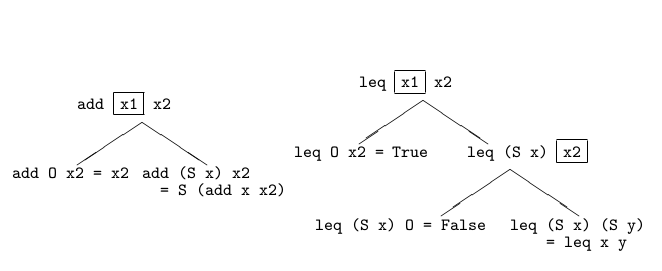
\includegraphics[scale=0.5]{pictures/def_trees.png}
  
\end{frame}

\begin{frame}

  Definitional Trees are particulary useful because they can be computed at compile time and they contain all infromation for the decisions to the steps in the rewriting process.

  We could define a needed narrowing step as an application to an operation-rooted term $t$ by considering it's definitional tree from the root. The tree is recursively processed until one finds a \textit{maximal} pattern that \textit{unifies} with $t$ (similarly with the M.G.U finding process in logic languages). From there (with the new tree) we perform the operation (at each node $\pi$ as it follows:

\end{frame}

\begin{frame}
  \begin{itemize}
    \setlength{\itemindent}{2cm}
\item[If $\pi$ is a leaf] we apply the corresponding rule
\item[If $\pi$ is a branch] let p be it's inductive position, we consider the corresponding subterm$t|_p$
  \begin{itemize}
    \item If $t|_p$ is rooted by a constructor $c$, if there is a child  with $c$ at the inductive position, we examine the child, else we fail.

    \item If $t|_p$ is a variable, we nondeterministaclly instantiate this variable by the constructor term at the inductive position of a child, and proceed to examine the child.

    \item If $t|_p$ is operation rooted, we recusively apply the computation of a needed narrowing step to $\sigma(t|_p)$, where $\sigma$ is the substution, result of previous case distinctions.
  \end{itemize}
\end{itemize}

\end{frame}
\end{subsection}
\begin{subsection}{Strict Equality}
\begin{frame}[fragile]
    The equality symbol \verb|=:=| is called \textit{strict equality}, i.e. te equation $t_1 =:= t_2$ is satisfied iff $t_1$ and $t_2$ are reducible to the same \textit{ground} constructor or term. (Note that when $t_1$ is not reducible, $t_1 =:= t_1$ does not succeed).

    We can define $=:=$ as follows:

    \[
    \begin{array}{llr}
    
      c =:= c &= \UseVerb{succ} &\forall  c/0\\
      c x_1 \ldots ~ x_n =:= c y_1 \ldots ~ y_n &= x_1 =:= y_1 ~\&~ \ldots x_n =:= y_n &\forall c/n \\
      \UseVerb{succ}~ \&~ \UseVerb{succ} &= \UseVerb{succ}
    \end{array}
    \]
\end{frame}

\begin{frame}[fragile]

A solution for an equation $t_1 =:= t_2$ is a substitution $\sigma$, if $\sigma(t_1) =:= \sigma(t_2) \leadsto^* \UseVerb{succ}$.

We have then, that \textit{needed narrowing} is Correct, Complete and Minimal (if there are two derivations, then their substitutions are independent). And, in successful derivations, needed narrowing computes the \textit{shortest} of al possible narrowing derivations.x

\end{frame}
\end{subsection}

\begin{subsection}{Weakly Needed Narrowing}

\begin{frame}[fragile]

  If we take the code:
\begin{verbatim}

or _ True = True
or True _ = True
or False False = False

\end{verbatim}

  We can see that the rule or doesn't have a definitional tree in the sense that when one of the arguments is True, it is not clear which rule should be evaluated. So we can extend the definition of \textit{inductivel sequential TRS} to a \textit{weakly orthogonal TRS} by requiring only that, for all variants of rules $\l_1 \rightarrow r_1$, $l_2 \rightarrow r_2$, if $\sigma(l_1) = \sigma(l_2)$ then $\sigma(r_1) = \sigma(r_2)$.

\end{frame}

\begin{frame}
  Then, we can also extend the definition of \textit{definitional trees} by adding or-branches, which are conceptually the union of two definitional trees.

  In the previous example, we could create a tree for the rules {$or_2,or_3$} and the rule {$or_1$}, then we could join those trees by an or-branch.

  This new way of resolving operations is also confluent, for the condition we required.

  \end{frame}
\end{subsection}

\begin{subsection}{Non-determinism}
\begin{frame}[fragile]
  This same principe may also be extended to handle non-deterministic operations and extra variables, by simply examining every possible or branch, and not requiring that all the rules are confluent to the same normal form. For example, the rule

\begin{verbatim}
x ? _ = x
_ ? y = y
\end{verbatim}

  Gives two results for \verb|0 ? 1|, namely \verb|0| and \verb|1|.
  
\end{frame}

\end{subsection}
\end{section}
\begin{section}{Bibliography}
  \begin{frame}
    \begin{itemize}
    \item Curry: A tutorial Introduction. Draft of December 2007. Antoy Sergio, Hanus Michael, Taken from http://www.informatik.uni-kiel.de/~curry/tutorial/ the 15th of April, 2013.


    \item Functional Logic Programming: From Theory to Curry. Hanus Michale. Institut f\"ur Informatik, CAU Kiel, Germany. As sent May the 13th of 2013.

    \item Curry An integrated functional language. September 11,2012. Hanus Michael, retrieved the 15th of April 2013.
      
    \end{itemize}

\end{frame}
\end{section}

\end{document}
